\chapter{Introduzione}
\label{cap:introduzione}

%Introduzione al contesto applicativo.\\

%\noindent Esempio di utilizzo di un termine nel glossario \\
%\gls{api}. \\

%\noindent Esempio di citazione in linea \\
%%\cite{site:agile-manifesto}. \\

%\noindent Esempio di citazione nel pie' di pagina \\
%citazione\footcite{womak:lean-thinking} \\

In questa sezione vengono descritte l'azienda ospitante, il \emph{device} utilizzato durante il tirocinio e gli strumenti di sviluppo e comunicazione utilizzati.

\section{Euronovate Group}
\begin{figure}[!h] 
    \centering 
    
\includegraphics[width=300pt]{images/euronovateGroupLogo.png} 
    \caption{Logo Euronovate Group}
    \label{fig:euronovateLogo}
\end{figure}
\emph{Euronovate Group} è un gruppo multinazionale con oltre 150 dipendenti, leader nel mercato
nell'implementazione e commercializzazione di soluzioni innovative per la trasformazione digitale,
Certification Authority eIDAS compliant, e produttrice di oltre 50 prodotti proprietari HW e
SW.\\
Ha sede centrale a Mendrisio (Svizzera) e controllate con presenza diretta in 4 paesi:
\begin{itemize}
    \item Italia (Padova, Reggio Emilia, Milano)
    \item Spagna (Barcellona, Madrid, Bilbao)
    \item Romania (Bucarest)
    \item Cina (Shanghai)
\end{itemize}
Euronovate Group inoltre si suddivide in:
\begin{itemize}
    \item Euronovate SA
    \item eSignWorld
    \item Vintegris
\end{itemize}

\subsection{Euronovate SA}
Fondata nel 2012 e con sede a Lugano (CH), è una società svizzera innovativa, leader in soluzioni
di Digital Trasformation con approccio end-to-end, combinando soluzioni software, hardware
e servizi di consulenza.\\
L'obiettivo principale è aiutare ogni tipo di azienda ad eliminare tutti i processi e i documenti
cartacei passando completamente al digitale, garantendo la stessa validità legale.
\subsection{eSignWorld}
Società che opera el settore della consulenza IT, processi e sistemi avanzati di firme elettroniche,
fornitura, esercizio e manutenzione di sistemi informativi hardware e software, specializzata nel
campo della produzione a filiera corta di tecnologia grafometrica.\\ In particolare, eSignWorld
fornisce soluzioni personalizzate e proprietarie nel campo della dematerializzazione documentale
e dell'Information Communication Technology, garantendo la possibilità di visualizzare,
elaborare e firmare elettronicamente qualsiasi tipo di documento.\\ eSignworld offre soluzioni
paperless con utilizzo di firma elettronica semplice e firma elettronica avanzata, un sistema di
composizione e successiva conservazione di documenti in formato elettronico, nonché di firma dei
documenti, attraverso un innovativo dispositivo di firma.
\subsection{Vintegris}
Víntegris progetta, implementa e gestisce infrastrutture di sicurezza per istituzioni finanziarie
e grandi società.\\ Fornisce solide soluzioni su misura per ogni esigenza di business, integrando
tecnologie ad alte prestazioni e soddisfacendo le esigenze di ogni azienda.\\ La società definisce e
realizza progetti ad alto valore aggiunto per la protezione delle informazioni, la sicurezza web, il
controllo e la gestione degli accessi.\\ Vengono utilizzate tecnologie tra le più robuste sul mercato
(Docker, Kubernetes, AWS, HSM), integrandole nell'ambiente aziendale di ciascun cliente.\\ L'es-
sere consulenti e integratori, pone Víntegris in una posizione privilegiata nello sviluppo di nuovi
prodotti: la conoscenza delle esigenze e delle criticità delle grandi aziende in materia di sicurezza
delle informazioni, guida Víntegris verso la progettazione di prodotti che coprono il divario tra le
soluzioni di sicurezza dei grandi produttori e le reali esigenze aziendali.\\ In questo modo, l'azienda
è in grado di anticipare le esigenze di mercato in segmenti critici come la gestione, il controllo e
gli audit di certificati digitali e autenticazione dell'utente.\\ Tutti i consulenti di Víntegris hanno
una vasta esperienza nel campo della tecnologia dell'informazione e sono esperti nella progetta-
zione, implementazione e gestione di infrastrutture di sicurezza delle informazioni.\\ Inoltre, la
maggior parte dei consulenti è in possesso di certificazioni riconosciute a livello internazionale,
come CISA, CISSP e CISM, che garantiscono la loro esperienza e conoscenza nell'ambito della
sicurezza delle informazioni.

\section{ENSign 11}

\begin{figure}[!h] 
    \centering 
    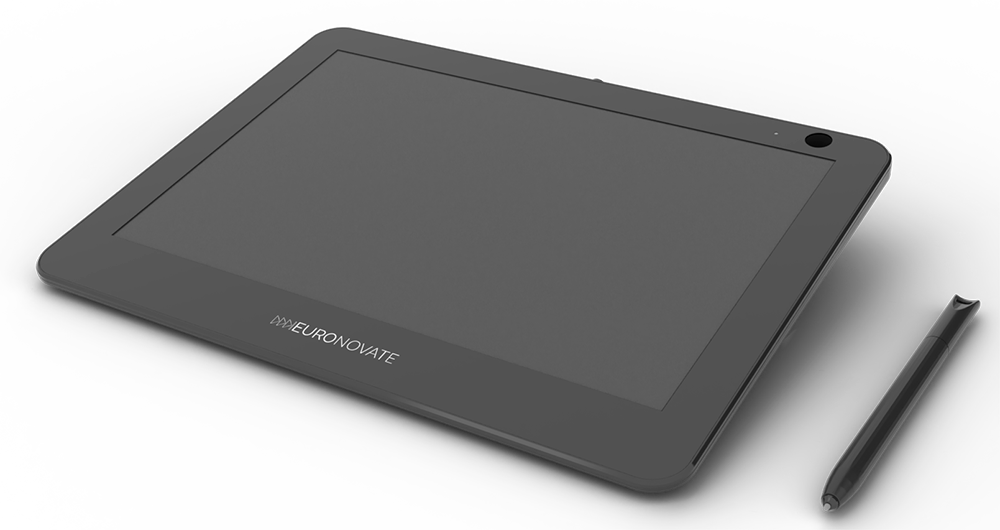
\includegraphics[width=300pt]{images/ensign11.png} 
    \caption{ENSign 11}
    \label{fig:ens11}
\end{figure}

L'ENSign 11 è un tablet versatile per firme grafometriche. Con le sue differenti applicazioni, è lo strumento perfetto per la digitalizzazione delle firme a mano.\\
L'ENSign è dotato delle seguenti caratteristiche:
\begin{itemize}
    \item pannello multi-tocco con isolamento nativo dello schermo
    \item connessione diretta ad un computer
    \item altamente compatto, con grande stabilità, alti livelli di sicurezza e design elegante
    \item cattura di parametri biometrici come pressione, accelerazione, velocità, ritmo e movimento in aria
    \item sistema proprietario di criptazione per ogni tipo di transazione
\end{itemize}
Inoltre, la versatilità dell'ENSign 11 permette di trasformarlo in un secondo schermo, semplicemente collegandolo tramite USB ad un computer e installando l'apposita applicazione ENSIGN 11 trayApp, in modo da avere tutte le funzionalità multimediali.\\
Con lo schermo multi-touch di ENSign 11 è possibile creare, scrivere, disegnare e mostrare contenuti multimediali personalizzati in tempo reale, che possono essere automaticamente condivisi attraverso videoconferenze o in presentazioni d'affari.

\section{Strumenti di comunicazione utilizzati}

Durante il tirocinio, sono stati utilizzati i seguenti strumenti di comunicazione:
\begin{itemize}
    \item \textbf{Gmail}, per le comunicazioni formali, quali la validazione dei documenti prodotti.
    \item \textbf{Google Meet}, per gli allineamenti durante le varie fasi del progetto.
    \item \textbf{Telegram}, per le comunicazioni informali.
    \item \textbf{Trello}, per la pianificazione delle attività settimanali (o per fase, se la durata è inferiore a 7 giorni).
\end{itemize}

\section{Strumenti di sviluppo}
\label{sec:sviluppoStrum}
\subsection{Sistema operativo}
L'azienda non ha imposto un determinato sistema operativo per lo sviluppo del progetto,in quanto non determinante per la buona riuscita dello stesso, dunque la mia scelta è ricaduta su Windows 11, in quanto è la versione più recente del famoso sistema operativo di casa Microsoft. Inoltre, essendo utilizzato da circa il 28\% degli utenti mondiali \footcite{site:statOS}, ha un ampio supporto sia ufficiale che non per l'installazione e la risoluzione di problemi all'interno dello stesso.
\subsection{Ambiente di sviluppo integrato}
Anche in questo caso, veniva lasciato allo stagista la scelta di un \gls{ideg}, ovvero di un ambiente di sviluppo integrato. La mia scelta è ricaduta su Visual Studio Code, sia per motivi di famigliarità sia per la varietà di tecnologie che il progetto richiedeva di utilizzare. Infatti, grazie alle numerevoli estensioni, Visual Studio Code è adatto per la programmazione con qualunque linguaggio esistente.
\subsection{Strumento per la creazione di documenti}
Dovendo creare dei documenti, era inoltre necessario scegliere uno strumento che ne permettesse la creazione. In questo caso, la mia scelta è caduta su \gls{latex}, in quanto avendolo utilizzato in ambito accademico è un linguaggio che ho apprezzato. Per l'installazione, ho utilizzato MiKTex, che ne permette l'installazione sui sistemi Windows, e ho utilizzato Visual Studio Code per l'utilizzo di questo linguaggio.

\section{Organizzazione del testo}
Il documento è strutturato nella seguente forma:
\begin{description}
    \item[{\hyperref[cap:introduzione]{Questo capitolo}}] ha fornito una descrizione generale sull'azienda, sul dispositivo oggetto del tirocinio e ha citato gli strumenti di sviluppo e comunicazione utilizzati.
    
    \item[{\hyperref[cap:descrizione-stage]{Il secondo capitolo}}] approfondisce in dettaglio in cosa consiste l'ENGaming.
    
    \item[{\hyperref[cap:analisi-requisiti]{Il terzo capitolo}}] illustra i requisiti che l'ENGaming affronta.
    
    \item[{\hyperref[cap:progettazione-codifica]{Il quarto capitolo}}] mostra come l'ENGaming garantisce la soddisfazione dei requisiti.
    
    \item[{\hyperref[cap:verifica-validazione]{Il quinto capitolo}}] indica come si garantisce che il prodotto sviluppato, in questo caso l'ENGaming, rispetti i requisiti definiti.
    
    \item[{\hyperref[cap:conclusioni]{Nel sesto capitolo}}] si conclude, dando una visione di massima di questo progetto.
\end{description}

%Riguardo la stesura del testo, relativamente al documento sono state adottate le seguenti convenzioni tipografiche:
%\begin{itemize}
%	\item gli acronimi, le abbreviazioni e i termini ambigui o di uso non comune menzionati vengono definiti nel glossario, situato alla fine del presente documento;
%	\item per la prima occorrenza dei termini riportati nel glossario viene utilizzata la seguente nomenclatura: \emph{parola}\glsfirstoccur;
%	\item i termini in lingua straniera o facenti parti del gergo tecnico sono evidenziati con il carattere \emph{corsivo}.
%\end{itemize}
